In this section, we explore the problem of detecting double compact objects with LISA analytically, focussing specifically on BHNS binaries, before presenting our full simulation results in Section~\ref{sec:resultsII}.

\subsection{The Role of Eccentricity}\label{sec:eccentricity_role}

Unlike BHBH binaries, a significant fraction of the BHNS binary population is highly eccentric. A high eccentricity has two major effects on detecting a binary with gravitational waves.

Firstly, eccentricity enhances the rate of energy emission via gravitational waves by a factor
\begin{equation}
    F(e) = \frac{1 + (73 / 24) e^2 + (37 / 96) e^4}{(1 - e^2)^{7/2}},
\end{equation}
compared to a circular binary with the same semi-major axis \citep[][Eq.\,17]{Peters+1963}. This means that eccentric binaries will not only inspiral faster, but also produce gravitational waves with stronger strain amplitudes (when summed over all harmonics).

Secondly, eccentric binaries will emit gravitational waves at many harmonic frequencies (unlike circular binaries, which only emit at twice the orbital frequency). This leads to the gravitational wave signal being diluted over many frequencies higher than the orbital frequency, where the higher the eccentricity, the more harmonics are required to capture all of the gravitational luminosity \citep[see][Fig.\,3]{Peters+1963}.

Therefore, though the first effect always increases the strength of the signal, the two effects in tandem do not necessarily always increase the detectability of a binary and we illustrate this point in Fig.\,\ref{fig:ecc_effects}. We show effect of eccentricity on the gravitational wave signal from a typical BHNS binary of chirp mass $\mathcal{M}_c = 3 \unit{M_{\odot}}$ and distance $8 \unit{kpc}$ at an orbital frequency of $f_{\rm orb} = 3 \times 10^{-4} \unit{Hz}$. Increasing the eccentricity from $e = 0.0$ to $0.5$ results in an increase in the signal-to-noise ratio (annotated on each set of points). This is because the eccentricity not only increases the gravitational wave emission, but also shifts the peak of the signal towards the minimum of the LISA sensitivity curve. However, further increasing the eccentricity from $e = 0.5$ to $0.9$ instead \textit{decreases} the signal-to-noise ratio. Although the greater eccentricity produces a stronger strain, it also shifts the peak of the gravitational wave signal to such high frequencies that the noise level is much higher and therefore has a lower signal-to-noise ratio.

Overall, we can therefore conclude that for BHNS binaries, higher eccentricity will produce more detectable binaries only if the orbital frequency is not already at or above the minimum of the LISA sensitivity curve. Another consideration for more massive binaries is whether the increased eccentricity will cause the binary to merge before the mission ends, which would cause a significant decrease in signal-to-noise ratio.

\begin{figure}[htb]
    \centering
    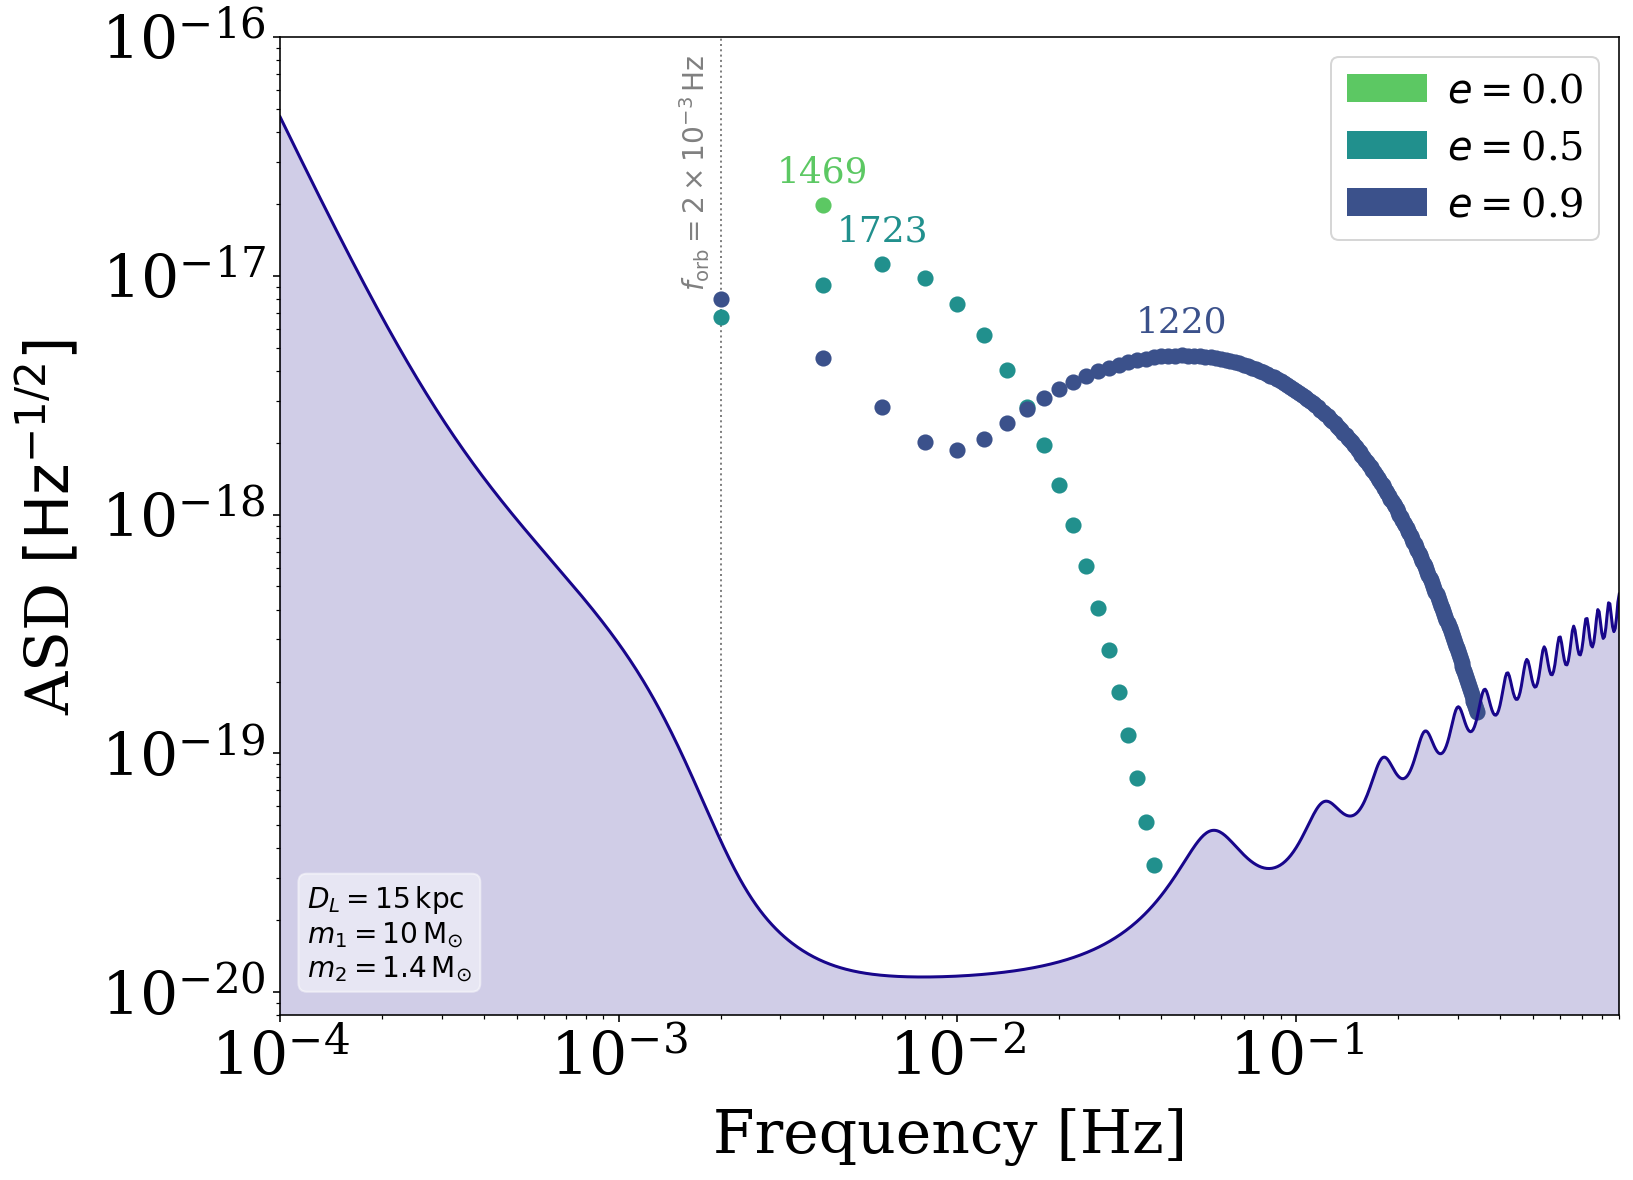
\includegraphics[width=\columnwidth]{e_sc_combined.png}
    \caption{An illustration of the effect of eccentricity on the detectability of a typical BHNS binary. Each point shows the strength of the gravitational wave signal at a harmonic frequency. We annotate each set of points with the binary's total signal-to-noise ratio summed over all harmonics and overplot the LISA sensitivity curve \citep{Robson+2019}.}
    \label{fig:ecc_effects}
\end{figure}

\subsection{Horizon Distance}

We define the horizon distance as the maximum distance at which a binary will have an signal-to-noise ratio above 7. In Figure~\ref{fig:bhns_horizon_distance} we show the horizon distance for a typical BHNS binary for different orbital frequencies and eccentricities. The horizon distance increases with frequency since the signal-to-noise ratio scales as
\begin{equation}
    \rho \propto \frac{N_{\rm cycle} \cdot h}{S_{\rm n}(f)} \propto \frac{f^{2/3} \cdot f^{1/2}}{S_{\rm n}(f)} \propto \frac{f^{7/6}}{S_{\rm n}(f)}.
\end{equation}
Since the minimum in the sensitivity curve occurs at $f \sim 10^{-2} \unit{Hz}$, the horizon distance increases monotonically with frequency. The dependence of the horizon distance on eccentricity follows the trends that we outlined in Section~\ref{sec:eccentricity_role}. The horizon distance increases with eccentricity up to a maximum, before decreasing once the eccentricity moves the peak of the gravitational wave luminosity past the minimum of the sensitivity curve. The eccentricity at which this maximum occurs is lower for higher orbital frequencies as less eccentricity is needed to move the peak past the minimum in the sensitivity curve. One may also note the sharp decrease in the horizon distance for binaries to the right of the $T_{\rm obs}$ contour, since these binaries will merge before the LISA mission is over.

This plot shows that, in principle, we could detect a BHNS binary up to several Mpc from Earth and thus plausibly in any galaxy in the Local Group. In reality, the number extragalactic detections will likely be very low since the binary needs to be very close to merging to be visible at that distance (as can be noted from the inspiral contours in Fig.~\ref{fig:bhns_horizon_distance}) and it is unlikely that a binary happen to be that close to merging during the LISA mission. However, more specific to this study, one can note that the combination of frequency and eccentricity required to be visible within the Milky Way (to the right of the white line in Fig.~\ref{fig:bhns_horizon_distance}) is much more probable.

\begin{figure}[htb]
    \centering
    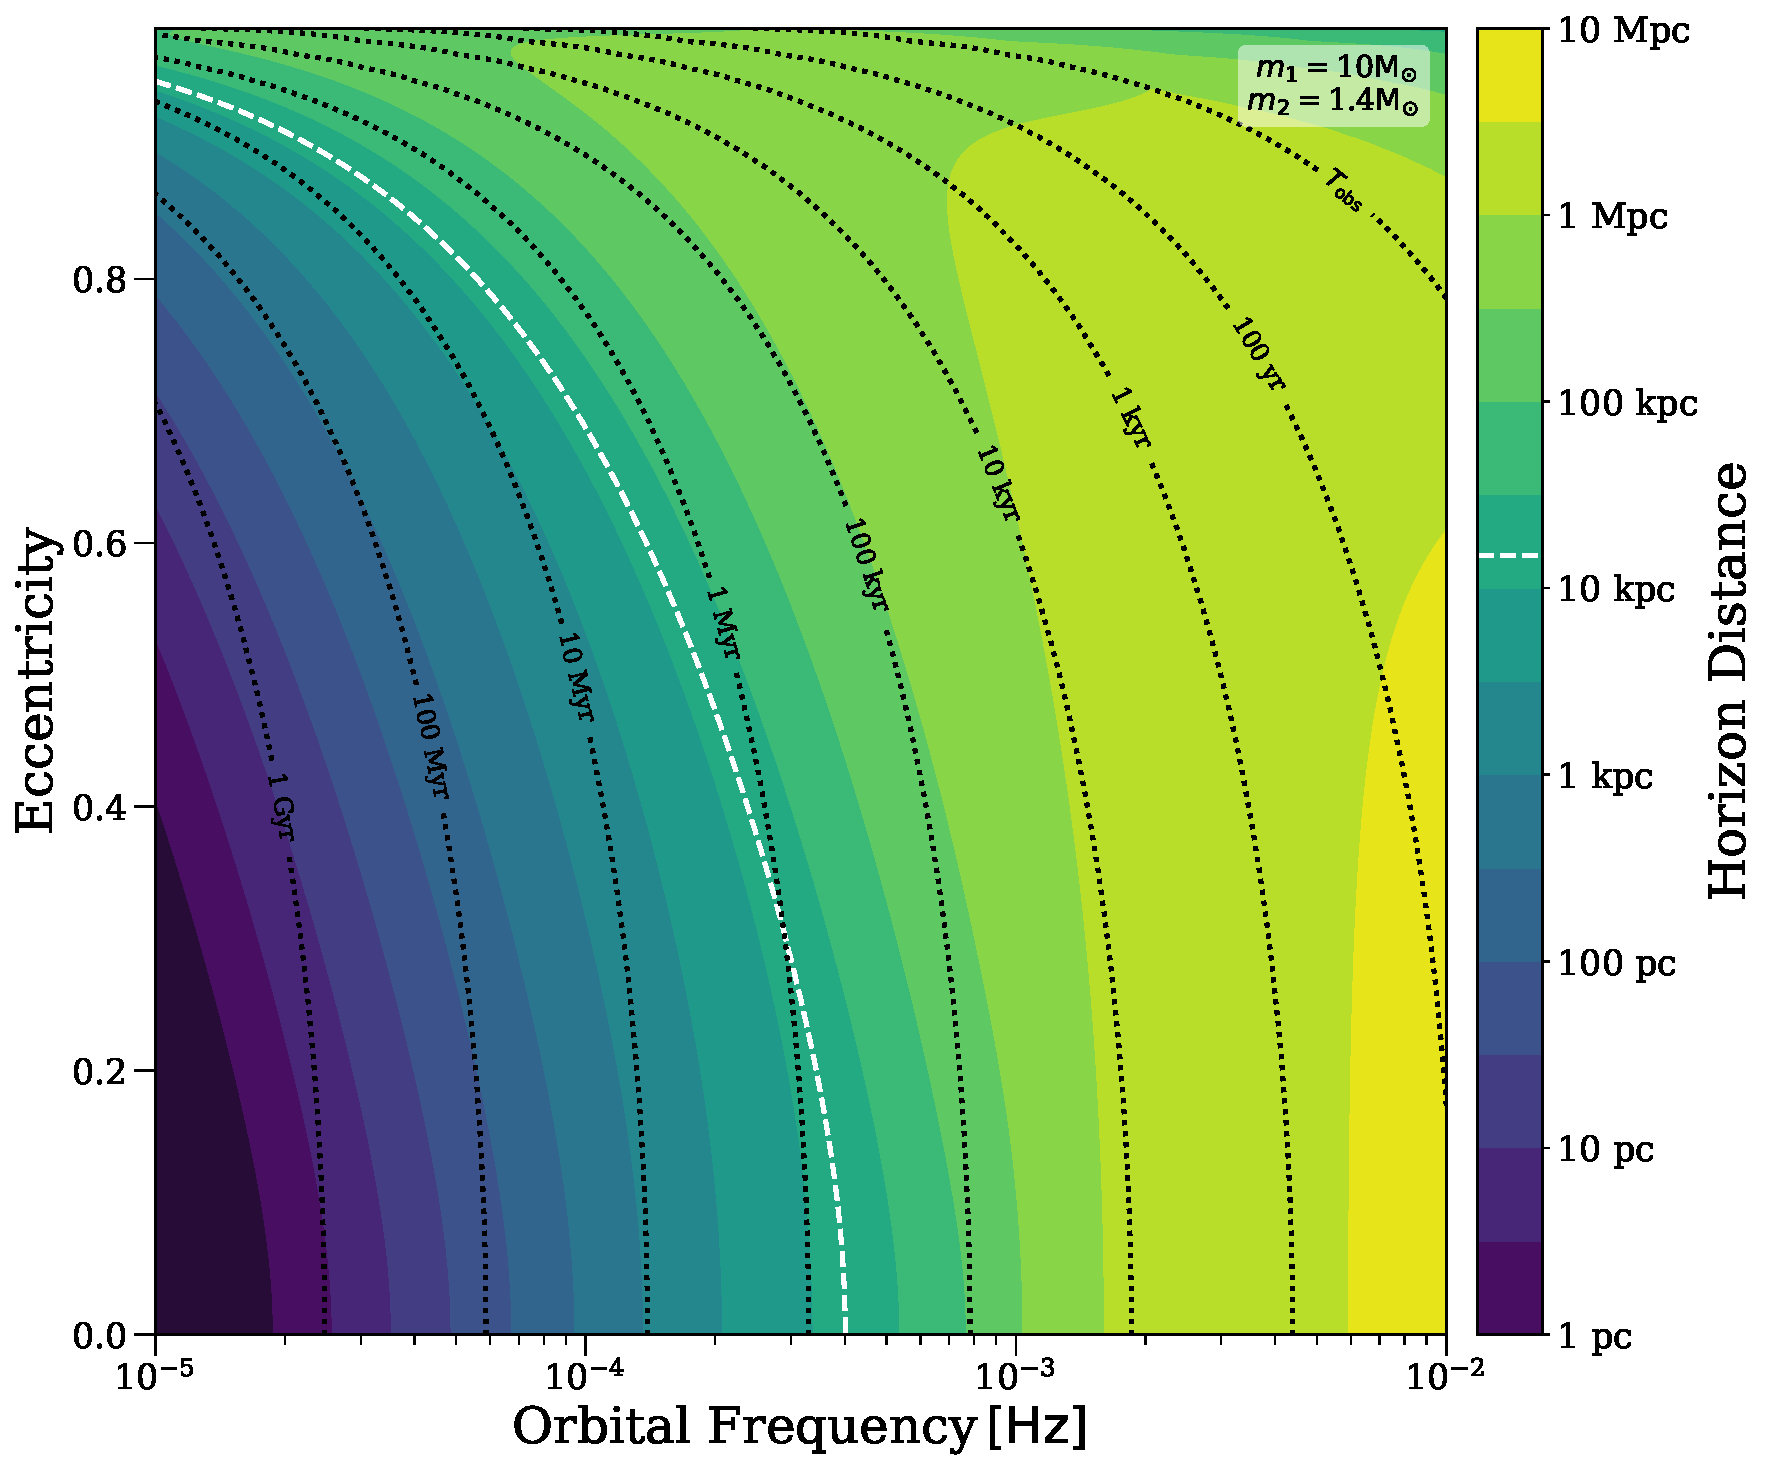
\includegraphics[width=\columnwidth]{horizon_distance.pdf}
    \caption{The horizon distance for a typical BHNS binary at different initial orbital frequencies and eccentricities is shown in the filled contours. The dashed white line indicates the edge of the Milky Way when using the \cite{Frankel+2018} model, which we define as the distance within which 99\% of binaries are contained. The dotted black lines show the inspiral time for the binary.}
    \label{fig:bhns_horizon_distance}
\end{figure}